\documentclass[12pt,a4paper]{report}
\usepackage[top=2.5cm,bottom=2.5cm,left=1.5cm,right=1.5cm]{geometry}

\usepackage{cmap}
\usepackage{graphicx}
\usepackage[english,slovak]{babel}
\usepackage[utf8]{inputenc}
\usepackage[T1]{fontenc}
%\usepackage{lmodern}

\usepackage{amssymb}
\usepackage{amsmath}

\usepackage{amsthm}
\newtheorem{veta}{Veta}[section]
\newtheorem{lema}[veta]{Lema}
\theoremstyle{definition}
\newtheorem{definicia}{Definícia}[chapter]
\theoremstyle{remark}
\newtheorem*{poznamka}{Poznámka}

\usepackage{setspace}
\onehalfspacing

\begin{document}

%\includepdf{zadanie.pdf}

%%% DEFINÍCIE NÁZVOV
\def\nazov{ŠPECIFIKÁCIA POŽIADAVIEK NA SOFTVÉR}
\def\autorJ{Jaroslav Fúska }
\def\autorT{Tomáš Sláma }
\def\autorH{ Martin Heinz }
\def\autorM{Michal Puškel }
\def\fakulta{Fakulta matematiky, fyziky a~informatiky}
\def\univerzita{Univerzita Komenského v~Bratislave}
\def\mesto{Bratislava}
\def\typprace{Športový klub}
\def\rok{2016}
%%% OBAL
\thispagestyle{empty}
\begin{center}
\textsc{\LARGE\univerzita}\\
\bigskip\textsc{\LARGE\fakulta}\\
\vfill\textsc{\Huge\nazov}\\
\medskip{\Large\typprace}\\
\vfill{\large\rok\hfill\autorJ\\ \hfill\autorT \\ \hfill \autorH \\ \hfill \autorM}
\end{center}

\tableofcontents

\chapter{Úvod}
%\setcounter{page}{5}
\addcontentsline{toc}{chapter}{\numberline {}Úvod}

\section{Predmet špecifikácie}
Táto špecifikácia požiadaviek na softvér (ďalej ŠPS) popisuje používateľské, funkčné a parametrické požiadavky prvej verzie systému pre webovú aplikáciu športového klubu. ŠPS je určená pre tím, ktorý bude výsledný   softvér   implementovať.  Špecifikácia   je   súčasťou   zmluvy   medzi   objednávateľom a dodávateľom.  Bude slúžiť ako  východisko  pre vyhodnocovanie správnosti softvéru.

\section{Rozsah projektu a funkcie systému}
Webový systém pre športový klub, bude vo svojej verzii poskytovať prostredie pre zaznamenávanie si bežeckých výkonov a správu a administráciu užívateľov. Úlohou tohto systému bude umožniť deťom priebežne si zaznamenávať ich bežecké výkony a zároveň ich motivovať pomocou vyobrazenej mapy s cieľom na daný mesiac. Administrátor a tréneri budú môcť spravovať uživateľov a vytvárať tímy. Pre každého použivateľa bude možné zobraziť históriu výkonov jeho aj celej jeho skupiny.

\section{Slovník pojmov, Skratky}

\begin{tabular}{ll}
\hline
\multicolumn{1}{|l|}{\shortstack{používateľ} }    & \multicolumn{1}{l|}{\shortstack[l]{osoba(dieťa), ktorá si môže zapisovať do aplikácie svoje výkony,\\ upravovať svoj profil a prehliadať históriu svojich výkonov}} \\ \hline
\multicolumn{1}{|l|}{administrátor} & \multicolumn{1}{l|}{osoba, ktorá môže potvrdzovať nových užívateľov, spravovať skupiny a oznamy}                                                  \\ \hline
\multicolumn{1}{|l|}{tréner}        & \multicolumn{1}{l|}{osoba, ktorá môže spravovať skupiny, ktoré trénuje a písať oznamy}                                                            \\ \hline
\multicolumn{1}{|l|}{výkon}         & \multicolumn{1}{l|}{nabehané kilometre a "pocit z behu"}                                                                                          \\ \hline

\end{tabular}
\newpage

\chapter{Celkový opis}

\section{Kontext systému}
Webová aplikácia predstavuje nový systém pre športový klub. So systémom pracuje používateľ, ktorý si zapisuje svoje bežecké výkony. Aplikácia komunikuje s databázou, v ktorej sa uchovávajú informácie o používateľoch. Aplikácia vytvára mapu s určitím vytýčeným cielom.

\subsection{Systémové rozhrania}

\begin{tabular}{ll}
\hline
\multicolumn{1}{|l|}{SR-1 }    & \multicolumn{1}{l|}{\shortstack[l]{Web aplikácia bude postavená na Open Source \\ technológiách PHP a databáze(SQLite), Javascript, CSS(LESS).}} \\ \hline
\multicolumn{1}{|l|}{SR-1.1} & \multicolumn{1}{l|}{\shortstack[l]{Web aplikácia musí korektne fungovať v prehliadačoch \\ Internet Explorer 10+, Firefox, Opera 11+ a Google Chrome}.}                                                  \\ \hline
\multicolumn{1}{|l|}{SR-2}        & \multicolumn{1}{l|}{Aplikácia vykonáva dopyty na Google Maps API}                                                            \\ \hline
\multicolumn{1}{|l|}{SR-2.1}         & \multicolumn{1}{l|}{Aplikácia vykonáva autentifikáciu uživatelov pomocou Google účtou.}                                                                                          \\ \hline

\end{tabular}

\subsection{Používateľské rozhrania}

\begin{tabular}{ll}
\hline
\multicolumn{1}{|l|}{PR-1 }    & \multicolumn{1}{l|}{\shortstack[l]{Používateľské rozhranie musí byť vytvorené formou web aplikácie.}} \\ \hline
\multicolumn{1}{|l|}{PR-2} & \multicolumn{1}{l|}{\shortstack[l]{Aplikácia bude responzívna(bude prispôsobená pre mobilné zariadenia)}.}                                                  \\ \hline
\multicolumn{1}{|l|}{PR-3}        & \multicolumn{1}{l|}{Používateľské rozhranie bude rozdelené na užívateľskú a správcovskú časť.}                                                            \\ \hline

\end{tabular}

\subsection{Hardvérové rozhrania}
Systém neobsahuje žiadne hardvérové rozhrania.

\subsection{Komunikačné rozhrania}
\begin{tabular}{ll}
\hline
\multicolumn{1}{|l|}{KR-1 }    & \multicolumn{1}{l|}{\shortstack[l]{Po registrácii pošle systém uživateľovi potvrdzovací e-mail}} \\ \hline
\end{tabular}


\section{Funkcie systému}
Prehľad funkcií, ktoré webový systém poskytuje používateľovi (Administrátorovi, Trénerovi a Bežcovi) je zobrazený na Obrázku 2.1.  \\

\begin{figure}[ht!]
\centering
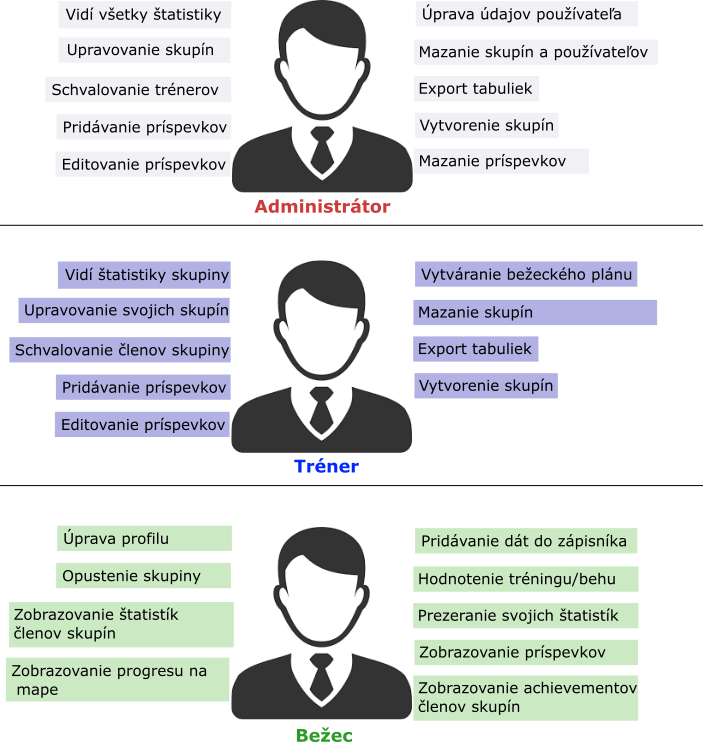
\includegraphics[width=130mm]{diagram.png}
\caption{Návrh funkcií systému \label{overflow}}
\end{figure}

\section{Triedy používateľov a ich vlastnosti}

\begin{tabular}{ll}
\hline
\multicolumn{1}{|l|}{Administrátor}    & \multicolumn{1}{l|}{\shortstack[l]{Používateľ s maximálnymi možnými právomocami na správu webovej \\ aplikácie, používateľov a skupín. Úlohou administrátora je dohliadať na \\ používateľov, pomáhať s riešením problémov, starať sa o aktuálnosť \\ informacií, schvaľovanie nových trénerov a prípadná editácia skupín a \\ používateľov.}} \\ \hline
\multicolumn{1}{|l|}{Tréner} & \multicolumn{1}{l|}{\shortstack[l]{Tréner musí byť schválený administrátorom. Jeho úlohou je spravovať \\ svoje skupiny, vytvárať bežecké plány a pridávať aktuality týkajúce \\ sa športového klubu.}}                                                  \\ \hline
\multicolumn{1}{|l|}{Bežec}        & \multicolumn{1}{l|}{\shortstack[l]{Koncový používateľ webovej aplikácie pre koho je určená. Má prístup \\ k prihláseniu, zapisovaniu svojich výsledkov do zápisníka, sledovaniu \\ svojho progresu a achievementov, prezeraniu svojich štatistík. Bežec \\ si môže prezerať profil iného bežca zo svojej skupiny. Svoj profil môže \\ kedykoľvek editovať.}                          }                                                                             \\ \hline
\end{tabular}

\section{Budúca verzia systému}
Zatiaľ nie sú plánované ďaľšie verzie systému.


\chapter{Špecifikácia požiadaviek}

\section{Možnosti bežca po prihlásení}

\subsection{Zobrazovanie príspevkov na domovskej stránke}
\begin{tabular}{ll}
\hline
\multicolumn{1}{|l|}{Popis:}    & \multicolumn{1}{l|}{\shortstack[l]{Používateľ bude mať možnosť vidieť všetky aktuálne príspevky a \\ oznamy od trénerov a administrátora. Nebudú mať možnosť ich \\ upravovať ani mazať. V prípade že chce bežec reagovať na príspevok \\ má  možnosť prekliknúť sa na profil prispievateľa a následne \\ ho kontaktovať e-mailom. }} \\ \hline
\multicolumn{1}{|l|}{Vstupné podmienky:} & \multicolumn{1}{l|}{\shortstack[l]{ - }}                                                  \\ \hline
\multicolumn{1}{|l|}{Výstupné podmienky:}& \multicolumn{1}{l|}{\shortstack[l]{-} }                                         \\ \hline
\multicolumn{1}{|l|}{Opakovanosť :} & \multicolumn{1}{l|}{\shortstack[l]{Ľubovoľná}}                                                  \\ \hline
\end{tabular}

\subsection{Zobrazovanie štatistík}
\begin{tabular}{ll}
\hline
\multicolumn{1}{|l|}{Popis:}    & \multicolumn{1}{l|}{\shortstack[l]{Používateľ bude mať možnosť vidieť tabuľku so svojími výkonmi.\\Bude si môcť vybrať aj tímové štatistiky, kde nebude vidieť \\ jednotlivých členov, ale výkon ako celku a koľkým \\i percentami prispel k tomuto výkonu. }} \\ \hline
\multicolumn{1}{|l|}{Vstupné podmienky:} & \multicolumn{1}{l|}{\shortstack[l]{- }}                                                  \\ \hline
\multicolumn{1}{|l|}{Výstupné podmienky:}& \multicolumn{1}{l|}{\shortstack[l]{-} }                                         \\ \hline
\multicolumn{1}{|l|}{Opakovanosť :} & \multicolumn{1}{l|}{\shortstack[l]{Ľubovoľná}}                                                  \\ \hline
\end{tabular}

\subsection{Vkladanie údajov do zápisníka}
\begin{tabular}{ll}
\hline
\multicolumn{1}{|l|}{Popis:}    & \multicolumn{1}{l|}{\shortstack[l]{Používateľovi sa zobrazí formulár, do ktorého zadá dátum, koľko \\ kilometrov zabehol, môže pridať komentár a  ohodnotiť tréning \\ pomocou smajlíkov. Po zadaní údajov sa kilometre pripočítajú \\ k tímovej štatistike a bežec bude môcť na mape sledovať o kolko \\ sa jeho tím posunul v napĺňaní svojho bežeckého\\ plánu k dosiahnutiu cieľa. }} \\ \hline
\multicolumn{1}{|l|}{Vstupné podmienky:} & \multicolumn{1}{l|}{\shortstack[l]{- }}                                                  \\ \hline
\multicolumn{1}{|l|}{Výstupné podmienky:}& \multicolumn{1}{l|}{\shortstack[l]{-} }                                         \\ \hline
\multicolumn{1}{|l|}{Opakovanosť :} & \multicolumn{1}{l|}{\shortstack[l]{Ľubovoľná}}                                                  \\ \hline
\end{tabular}

\subsection{Zobrazovanie Achievementov}
\begin{tabular}{ll}
\hline
\multicolumn{1}{|l|}{Popis:}    & \multicolumn{1}{l|}{\shortstack[l]{Bežec dostáva po splnení určeného cieľa (napr. zabehnúť spolu 50km)\\ achievement.  Čím viacej sa bežec snaží napredovať, tým výnimočnejší\\ achievement dostane, čo by ho malo motivovať k ďaľším výkonom.}} \\ \hline
\multicolumn{1}{|l|}{Vstupné podmienky:} & \multicolumn{1}{l|}{\shortstack[l]{ - }}                                                  \\ \hline
\multicolumn{1}{|l|}{Výstupné podmienky:}& \multicolumn{1}{l|}{\shortstack[l]{-} }                                         \\ \hline
\multicolumn{1}{|l|}{Opakovanosť :} & \multicolumn{1}{l|}{\shortstack[l]{Preddefinovaná}}                                                  \\ \hline
\end{tabular}

\subsection{Zobrazovanie profilu bežca}
\begin{tabular}{ll}
\hline
\multicolumn{1}{|l|}{Popis:}    & \multicolumn{1}{l|}{\shortstack[l]{Bežec má už po vyplnení registrácie svoj vlastný profil, \\ ktorý obsahuje základné informácie o bežcovi ako napr. meno,\\ vek, kontaktné údaje a fotku.\\ Bežec si môže prezerať aj profil iných členov skupiny a svojho trénera.}} \\ \hline
\multicolumn{1}{|l|}{Vstupné podmienky:} & \multicolumn{1}{l|}{\shortstack[l]{- }}                                                  \\ \hline
\multicolumn{1}{|l|}{Výstupné podmienky:}& \multicolumn{1}{l|}{\shortstack[l]{-} }                                         \\ \hline
\multicolumn{1}{|l|}{Opakovanosť :} & \multicolumn{1}{l|}{\shortstack[l]{Ľubovoľná}}                                                  \\ \hline
\end{tabular}

\subsection{Upravenie profilu}
\begin{tabular}{ll}
\hline
\multicolumn{1}{|l|}{Popis:}    & \multicolumn{1}{l|}{\shortstack[l]{Každý bežec môže upravovať svoj profil, teda vybrať si jedného \\ zo skupiny avatarov, zmeniť názov školy, \\ upraviť dátum narodenia, prípadne pridať kontaktné údaje. }} \\ \hline
\multicolumn{1}{|l|}{Vstupné podmienky:} & \multicolumn{1}{l|}{\shortstack[l]{ - }}                                                  \\ \hline
\multicolumn{1}{|l|}{Výstupné podmienky:}& \multicolumn{1}{l|}{\shortstack[l]{-} }                                         \\ \hline
\multicolumn{1}{|l|}{Opakovanosť :} & \multicolumn{1}{l|}{\shortstack[l]{Ľubovoľná}}                                                  \\ \hline
\end{tabular}

\subsection{Opustenie skupiny}
\begin{tabular}{ll}
\hline
\multicolumn{1}{|l|}{Popis:}    & \multicolumn{1}{l|}{\shortstack[l]{Každý bežec môže opustiť svoju skupinu. Po opustení skupiny \\ bude musieť požiadať trénera aby mu pridelil novú skupinu.}} \\ \hline
\multicolumn{1}{|l|}{Vstupné podmienky:} & \multicolumn{1}{l|}{\shortstack[l]{- }}                                                  \\ \hline
\multicolumn{1}{|l|}{Výstupné podmienky:}& \multicolumn{1}{l|}{\shortstack[l]{-} }                                         \\ \hline
\multicolumn{1}{|l|}{Opakovanosť :} & \multicolumn{1}{l|}{\shortstack[l]{Jednorázová}}                                                  \\ \hline
\end{tabular}

\section{Možnosti trénera po prihlásení}

\subsection{Zobrazenie štatistík skupiny}
\begin{tabular}{ll}
\hline
\multicolumn{1}{|l|}{Popis:}    & \multicolumn{1}{l|}{\shortstack[l]{Tréner bude mať možnosť zobrazovať štatistiky svojich skupín.}} \\ \hline
\multicolumn{1}{|l|}{Vstupné podmienky:} & \multicolumn{1}{l|}{\shortstack[l]{-}}                                                  \\ \hline
\multicolumn{1}{|l|}{Výstupné podmienky:}& \multicolumn{1}{l|}{\shortstack[l]{-} }                                         \\ \hline
\multicolumn{1}{|l|}{Opakovanosť :} & \multicolumn{1}{l|}{\shortstack[l]{Ľubovoľná}}                                                  \\ \hline
\end{tabular}

\subsection{Schvaľovanie členov skupiny}
\begin{tabular}{ll}
\hline
\multicolumn{1}{|l|}{Popis:}    & \multicolumn{1}{l|}{\shortstack[l]{Tréner bude mať možnosť schváliť alebo odmietnuť požiadavku \\ o vstup užívateľa do jeho skupiny. Požiadavka sa objaví po tom \\ ako si užívateľ vyberie svojho trénera. Každú požiadavku je \\ možné prijať/odmietnuť raz pre jeden užívateľov výber trénera.}} \\ \hline
\multicolumn{1}{|l|}{Vstupné podmienky:} & \multicolumn{1}{l|}{\shortstack[l]{Užívateľ pošle požiadavku pomocou výberu trénera}}                                                  \\ \hline
\multicolumn{1}{|l|}{Výstupné podmienky:}& \multicolumn{1}{l|}{\shortstack[l]{-} }                                         \\ \hline
\multicolumn{1}{|l|}{Opakovanosť :} & \multicolumn{1}{l|}{\shortstack[l]{V závislosti od požiadaviek.}}                                                  \\ \hline
\end{tabular}

\subsection{Pridávanie príspevkov na nástenku}
\begin{tabular}{ll}
\hline
\multicolumn{1}{|l|}{Popis:}    & \multicolumn{1}{l|}{\shortstack[l]{Tréner bude mať možnosť pridať príspevky na nástenku na \\ domovskej stránke aplikácie, ktoré budú viditeľné pre \\ prihlásených užívateľov.}} \\ \hline
\multicolumn{1}{|l|}{Vstupné podmienky:} & \multicolumn{1}{l|}{\shortstack[l]{-}}                                                  \\ \hline
\multicolumn{1}{|l|}{Výstupné podmienky:}& \multicolumn{1}{l|}{\shortstack[l]{-} }                                         \\ \hline
\multicolumn{1}{|l|}{Opakovanosť :} & \multicolumn{1}{l|}{\shortstack[l]{Ľubovoľná}}                                                  \\ \hline
\end{tabular}

\subsection{Editovanie príspevkov na nástenke}
\begin{tabular}{ll}
\hline
\multicolumn{1}{|l|}{Popis:}    & \multicolumn{1}{l|}{\shortstack[l]{Tréner bude mať možnosť editovať svoje príspevky na domovskej \\ stránke aplikácie.}} \\ \hline
\multicolumn{1}{|l|}{Vstupné podmienky:} & \multicolumn{1}{l|}{\shortstack[l]{-}}                                                  \\ \hline
\multicolumn{1}{|l|}{Výstupné podmienky:}& \multicolumn{1}{l|}{\shortstack[l]{-} }                                         \\ \hline
\multicolumn{1}{|l|}{Opakovanosť :} & \multicolumn{1}{l|}{\shortstack[l]{Ľubovoľná}}                                                  \\ \hline
\end{tabular}

\subsection{Vytváranie bežeckého plánu}
\begin{tabular}{ll}
\hline
\multicolumn{1}{|l|}{Popis:}    & \multicolumn{1}{l|}{\shortstack[l]{Tréner bude mať možnosť vytvoriť bežecký plán pre svoju skupinu \\ zvolením trasi na mape. Cieľom skupiny je spoločne odbehnúť počet \\ kilometrov určený touto trasou.}} \\ \hline
\multicolumn{1}{|l|}{Vstupné podmienky:} & \multicolumn{1}{l|}{\shortstack[l]{-}}                                                  \\ \hline
\multicolumn{1}{|l|}{Výstupné podmienky:}& \multicolumn{1}{l|}{\shortstack[l]{-} }                                         \\ \hline
\multicolumn{1}{|l|}{Opakovanosť :} & \multicolumn{1}{l|}{\shortstack[l]{Ľubovoľná}}                                                  \\ \hline
\end{tabular}

\subsection{Mazanie skupín}
\begin{tabular}{ll}
\hline
\multicolumn{1}{|l|}{Popis:}    & \multicolumn{1}{l|}{\shortstack[l]{Tréner bude mať možnosť zmazať svoju skupinu.}} \\ \hline
\multicolumn{1}{|l|}{Vstupné podmienky:} & \multicolumn{1}{l|}{\shortstack[l]{-}}                                                  \\ \hline
\multicolumn{1}{|l|}{Výstupné podmienky:}& \multicolumn{1}{l|}{\shortstack[l]{-} }                                         \\ \hline
\multicolumn{1}{|l|}{Opakovanosť :} & \multicolumn{1}{l|}{\shortstack[l]{Kým existuje aspoň jedna skupina vytvorená trénerom.}}                                                  \\ \hline
\end{tabular}

\subsection{Export tabuliek}
\begin{tabular}{ll}
\hline
\multicolumn{1}{|l|}{Popis:}    & \multicolumn{1}{l|}{\shortstack[l]{Tréner bude mať možnosť vyexportovať tabuľky so štatistikami \\ jeho skupiny.}} \\ \hline
\multicolumn{1}{|l|}{Vstupné podmienky:} & \multicolumn{1}{l|}{\shortstack[l]{-}}                                                  \\ \hline
\multicolumn{1}{|l|}{Výstupné podmienky:}& \multicolumn{1}{l|}{\shortstack[l]{-} }                                         \\ \hline
\multicolumn{1}{|l|}{Opakovanosť :} & \multicolumn{1}{l|}{\shortstack[l]{Ľubovoľná}}                                                  \\ \hline
\end{tabular}

\subsection{Vytvorenie skupín}
\begin{tabular}{ll}
\hline
\multicolumn{1}{|l|}{Popis:}    & \multicolumn{1}{l|}{\shortstack[l]{Tréner bude mať možnosť vytvoriť skupinu.}} \\ \hline
\multicolumn{1}{|l|}{Vstupné podmienky:} & \multicolumn{1}{l|}{\shortstack[l]{-}}                                                  \\ \hline
\multicolumn{1}{|l|}{Výstupné podmienky:}& \multicolumn{1}{l|}{\shortstack[l]{-} }                                         \\ \hline
\multicolumn{1}{|l|}{Opakovanosť :} & \multicolumn{1}{l|}{\shortstack[l]{Ľubovoľná}}                                                  \\ \hline
\end{tabular}

\section{Možnosti administrátora po prihlásení}

\subsection{Pridávanie príspevkov}
\begin{tabular}{ll}
\hline
\multicolumn{1}{|l|}{Popis:}    & \multicolumn{1}{l|}{\shortstack[l]{Administrátor bude mať možnosť pridávať príspevky a oznamy na hlavnú\\ stránku.}} \\ \hline
\multicolumn{1}{|l|}{Vstupné podmienky:} & \multicolumn{1}{l|}{\shortstack[l]{-}}                                                  \\ \hline
\multicolumn{1}{|l|}{Výstupné podmienky:}& \multicolumn{1}{l|}{\shortstack[l]{-} }                                         \\ \hline
\multicolumn{1}{|l|}{Opakovanosť :} & \multicolumn{1}{l|}{\shortstack[l]{Ľubovoľná}}                                                  \\ \hline
\end{tabular}

\subsection{Editovanie príspevkov}
\begin{tabular}{ll}
\hline
\multicolumn{1}{|l|}{Popis:}    & \multicolumn{1}{l|}{\shortstack[l]{Administrátor bude mať možnosť upravovať príspevky a oznamy na hlavnej\\ stránke. Ako jediný bude môcť upravovať aj príspevky trénerov.}} \\ \hline
\multicolumn{1}{|l|}{Vstupné podmienky:} & \multicolumn{1}{l|}{\shortstack[l]{-}}                                                  \\ \hline
\multicolumn{1}{|l|}{Výstupné podmienky:}& \multicolumn{1}{l|}{\shortstack[l]{-} }                                         \\ \hline
\multicolumn{1}{|l|}{Opakovanosť :} & \multicolumn{1}{l|}{\shortstack[l]{Ľubovoľná}}                                                  \\ \hline
\end{tabular}

\subsection{Mazanie príspevkov}
\begin{tabular}{ll}
\hline
\multicolumn{1}{|l|}{Popis:}    & \multicolumn{1}{l|}{\shortstack[l]{Administrátor bude mať možnosť mazať ľubovoľné príspevky a oznamy na \\hlavnej stránke, teda aj príspevky trénerov.}} \\ \hline
\multicolumn{1}{|l|}{Vstupné podmienky:} & \multicolumn{1}{l|}{\shortstack[l]{ -}}                                                  \\ \hline
\multicolumn{1}{|l|}{Výstupné podmienky:}& \multicolumn{1}{l|}{\shortstack[l]{-} }                                         \\ \hline
\multicolumn{1}{|l|}{Opakovanosť :} & \multicolumn{1}{l|}{\shortstack[l]{Kým existuje aspoň jeden príspevok}}                                                  \\ \hline
\end{tabular}

\subsection{Vytvorenie skupiny}
\begin{tabular}{ll}
\hline
\multicolumn{1}{|l|}{Popis:}    & \multicolumn{1}{l|}{\shortstack[l]{Administrátor bude mať možnosť podobne ako tréner vytvoriť skupinu,\\ ktorej pridelí trénera.}} \\ \hline
\multicolumn{1}{|l|}{Vstupné podmienky:} & \multicolumn{1}{l|}{\shortstack[l]{-}}                                                  \\ \hline
\multicolumn{1}{|l|}{Výstupné podmienky:}& \multicolumn{1}{l|}{\shortstack[l]{-} }                                         \\ \hline
\multicolumn{1}{|l|}{Opakovanosť :} & \multicolumn{1}{l|}{\shortstack[l]{Ľubovoľná}}                                                  \\ \hline
\end{tabular}

\subsection{Editovanie skupiny}
\begin{tabular}{ll}
\hline
\multicolumn{1}{|l|}{Popis:}    & \multicolumn{1}{l|}{\shortstack[l]{Administrátor bude mať možnosť upravovať skupinu.}} \\ \hline
\multicolumn{1}{|l|}{Vstupné podmienky:} & \multicolumn{1}{l|}{\shortstack[l]{-}}                                                  \\ \hline
\multicolumn{1}{|l|}{Výstupné podmienky:}& \multicolumn{1}{l|}{\shortstack[l]{-} }                                         \\ \hline
\multicolumn{1}{|l|}{Opakovanosť :} & \multicolumn{1}{l|}{\shortstack[l]{Ľubovoľná}}                                                  \\ \hline
\end{tabular}

\subsection{Mazanie skupiny}
\begin{tabular}{ll}
\hline
\multicolumn{1}{|l|}{Popis:}    & \multicolumn{1}{l|}{\shortstack[l]{Administrátor bude mať možnosť zmazať skupinu.}} \\ \hline
\multicolumn{1}{|l|}{Vstupné podmienky:} & \multicolumn{1}{l|}{\shortstack[l]{-}}                                                  \\ \hline
\multicolumn{1}{|l|}{Výstupné podmienky:}& \multicolumn{1}{l|}{\shortstack[l]{-} }                                         \\ \hline
\multicolumn{1}{|l|}{Opakovanosť :} & \multicolumn{1}{l|}{\shortstack[l]{Kým existuje aspoň jedna skupina}}                                                  \\ \hline
\end{tabular}

\subsection{Editovanie používateľa}
\begin{tabular}{ll}
\hline
\multicolumn{1}{|l|}{Popis:}    & \multicolumn{1}{l|}{\shortstack[l]{Administrátor bude mať možnosť upravovať údaje používateľa. Nebude môcť \\meniť email a heslo, nakoľko bude použité google api.}} \\ \hline
\multicolumn{1}{|l|}{Vstupné podmienky:} & \multicolumn{1}{l|}{\shortstack[l]{-}}                                                  \\ \hline
\multicolumn{1}{|l|}{Výstupné podmienky:}& \multicolumn{1}{l|}{\shortstack[l]{-} }                                         \\ \hline
\multicolumn{1}{|l|}{Opakovanosť :} & \multicolumn{1}{l|}{\shortstack[l]{Ľubovoľná}}                                                  \\ \hline
\end{tabular}

\subsection{Zmazanie používateľa}
\begin{tabular}{ll}
\hline
\multicolumn{1}{|l|}{Popis:}    & \multicolumn{1}{l|}{\shortstack[l]{Administrátor bude mať možnosť vymazať používateľa z databázy\\ používateľov.}} \\ \hline
\multicolumn{1}{|l|}{Vstupné podmienky:} & \multicolumn{1}{l|}{\shortstack[l]{-}}                                                  \\ \hline
\multicolumn{1}{|l|}{Výstupné podmienky:}& \multicolumn{1}{l|}{\shortstack[l]{-} }                                         \\ \hline
\multicolumn{1}{|l|}{Opakovanosť :} & \multicolumn{1}{l|}{\shortstack[l]{Kým existuje aspoň jeden používateľ}}                                                  \\ \hline
\end{tabular}

\subsection{Schvaľovanie trénerov}
\begin{tabular}{ll}
\hline
\multicolumn{1}{|l|}{Popis:}    & \multicolumn{1}{l|}{\shortstack[l]{Aby sa bežný používateľ mohol stať trénerom, musí jeho žiadosť\\ schváliť (alebo zamietnuť) administrátor.}} \\ \hline
\multicolumn{1}{|l|}{Vstupné podmienky:} & \multicolumn{1}{l|}{\shortstack[l]{-}}                                                  \\ \hline
\multicolumn{1}{|l|}{Výstupné podmienky:}& \multicolumn{1}{l|}{\shortstack[l]{-} }                                         \\ \hline
\multicolumn{1}{|l|}{Opakovanosť :} & \multicolumn{1}{l|}{\shortstack[l]{V závislosti od požiadaviek}}                                                  \\ \hline
\end{tabular}

\subsection{Zobrazovanie štatistík}
\begin{tabular}{ll}
\hline
\multicolumn{1}{|l|}{Popis:}    & \multicolumn{1}{l|}{\shortstack[l]{Administrátor, ako jediný, má možnosť vidieť štatistiky a výsledky\\ všetkých bežcov.}} \\ \hline
\multicolumn{1}{|l|}{Vstupné podmienky:} & \multicolumn{1}{l|}{\shortstack[l]{-}}                                                  \\ \hline
\multicolumn{1}{|l|}{Výstupné podmienky:}& \multicolumn{1}{l|}{\shortstack[l]{-} }                                         \\ \hline
\multicolumn{1}{|l|}{Opakovanosť :} & \multicolumn{1}{l|}{\shortstack[l]{Ľubovoľná}}                                                  \\ \hline
\end{tabular}

\subsection{Zobrazovanie profilov}
\begin{tabular}{ll}
\hline
\multicolumn{1}{|l|}{Popis:}    & \multicolumn{1}{l|}{\shortstack[l]{Administrátor, ako jediný, má možnosť vidieť profil každého bežca.}} \\ \hline
\multicolumn{1}{|l|}{Vstupné podmienky:} & \multicolumn{1}{l|}{\shortstack[l]{-}}                                                  \\ \hline
\multicolumn{1}{|l|}{Výstupné podmienky:}& \multicolumn{1}{l|}{\shortstack[l]{-} }                                         \\ \hline
\multicolumn{1}{|l|}{Opakovanosť :} & \multicolumn{1}{l|}{\shortstack[l]{Ľubovoľná}}                                                  \\ \hline
\end{tabular}

\subsection{Export tabuliek}
\begin{tabular}{ll}
\hline
\multicolumn{1}{|l|}{Popis:}    & \multicolumn{1}{l|}{\shortstack[l]{Administrátor bude mať možnosť vyexportovať tabuľky so štatistikami \\ ktorejkoľvek skupiny.}} \\ \hline
\multicolumn{1}{|l|}{Vstupné podmienky:} & \multicolumn{1}{l|}{\shortstack[l]{-}}                                                  \\ \hline
\multicolumn{1}{|l|}{Výstupné podmienky:}& \multicolumn{1}{l|}{\shortstack[l]{-} }                                         \\ \hline
\multicolumn{1}{|l|}{Opakovanosť :} & \multicolumn{1}{l|}{\shortstack[l]{Ľubovoľná}}                                                  \\ \hline
\end{tabular}


\chapter{Ďaľšie požiadavky}

\section{Výkonostné požiadavky}

\begin{itemize}  
\item Webová aplikácia bude spracovávať údaje členov jedného bežeckého klubu. 
\item Predpokladaný počet je maximálne 1000 členov
\item Počet dotazov na Google-maps api nepresiahne 2500/deň 
\end{itemize}

\section{Dostupnosť}
\begin{itemize}  
\item Dostupnosť servera aspoň 97\%
\end{itemize}

\section{Bezpečnostné požiadavky}
\begin{itemize}  
\item Zobrazenie profilov a obsahu až po registrácii alebo prihlásení
\item Na prihlasovanie používanie Google api
\item Schvaľovanie a kontrola administrátorom 
\item Obmedzené prístupové práva pre bežcov a trénerov
\end{itemize}



\end{document} 
